\documentclass[aspectratio=169, 11pt]{beamer}

\usetheme{CambridgeUS}
\usecolortheme{dolphin}

\usepackage[utf8]{inputenc}
\usepackage[L7x]{fontenc}
\usepackage[lithuanian]{babel}

\usepackage{amsmath}
\usepackage{amsfonts}
\usepackage{amssymb}
\usepackage{graphicx}


\usepackage{booktabs}
\usepackage{longtable}
\usepackage{array}
\usepackage{multirow}
\usepackage{wrapfig}
\usepackage{float}
\usepackage{colortbl}
\usepackage{pdflscape}
\usepackage{tabu}
\usepackage{threeparttable}
\usepackage{threeparttablex}
\usepackage[normalem]{ulem}
\usepackage{makecell}
\usepackage{xcolor}

\usepackage{hyperref}
\hypersetup{
  colorlinks=true,
  linkcolor=black,
  filecolor=blue,   
  urlcolor=blue,
  citecolor=blue
}

\author{Armintė G. Justas M. Tomas D.}
\title{COVID-19}
\subtitle{Skaičiai bei įžvalgos}
%\setbeamercovered{transparent} 
%\setbeamertemplate{navigation symbols}{} 
%\logo{} 
%\institute{Corona-Stat.lt} 
%\date{} 
%\subject{AAA} 

\graphicspath{{./figures/}}


\begin{document}

\begin{frame}
\titlepage
\end{frame}

\begin{frame}
\tableofcontents
\end{frame}

\section{Apie Corona-Stat.lt}
\begin{frame}{Corona-Stat.lt projektas}
\begin{itemize}
\item Corona-Stat.lt pirminis tikslas COVID19 plitimo prognozė
\item Komanda (Armintė, Rokas, Tomas)
\item SAM'o nulinė reakcija
\item Nuo COVID19 statistikos link ekonominių įžvalgų
\end{itemize}
\end{frame}


\begin{frame}{Apie COVID prognozavimą}
\begin{itemize}
\item Kaip prognozuojamos epi- ir pandemijos: SIR
\item $S \Longrightarrow I \Longrightarrow R$
\item Duomenų tikslumas (testavimo apimtis, latentinis periodas < inkubacinis periodas, asimptominis sirgimas, autopsijos)
\item \href{https://mif.vu.lt/lt3/dokumentai/dokumentai/Naujienos/COVID/2020-04-15_SEIR_ilgalakes_prognozes.pdf}{Lietuviški mokslininkai "prognozuoja"}
\end{itemize}
\centering
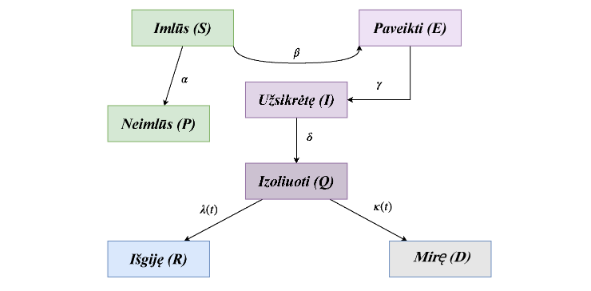
\includegraphics[scale=0.4]{seiqrdp.png}

\end{frame}

\section{Covid situacija}

\begin{frame}{Covid situacija - pasaulis}
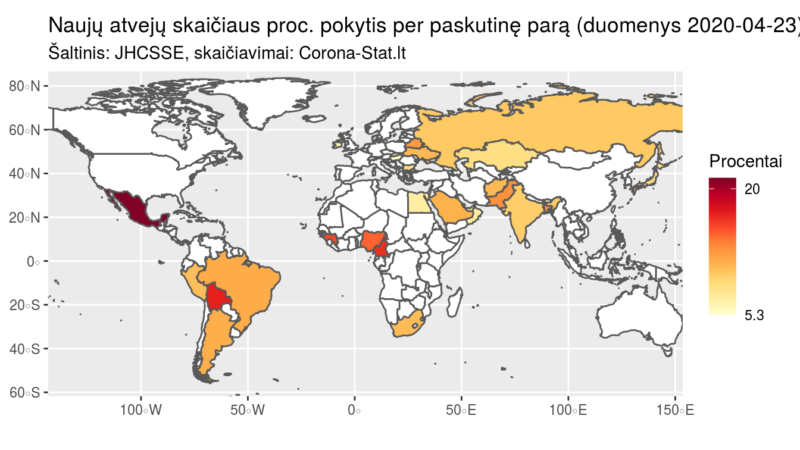
\includegraphics[scale=0.5]{world.png}
\end{frame}

\begin{frame}{Covid situacija - Europa}
\centering
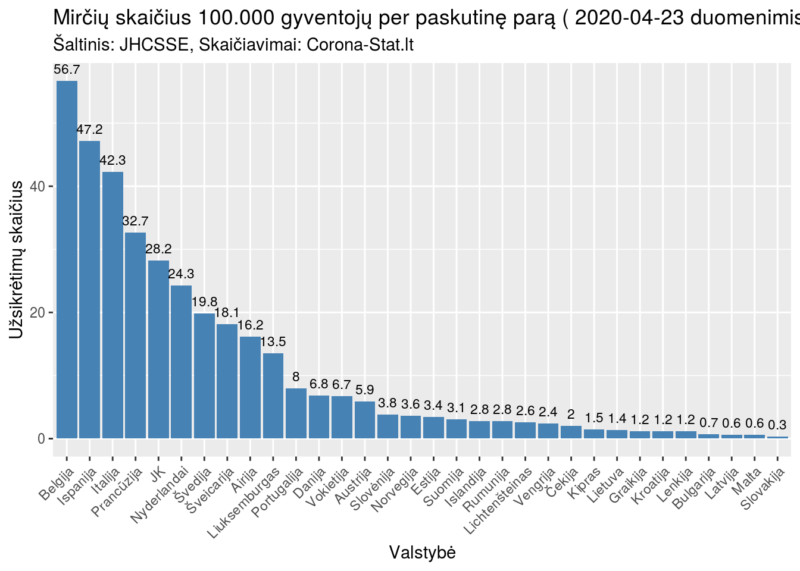
\includegraphics[scale=0.375]{mirtys_eu_pop.png}
\end{frame}

\begin{frame}{Covid situacija - Europa}
\centering
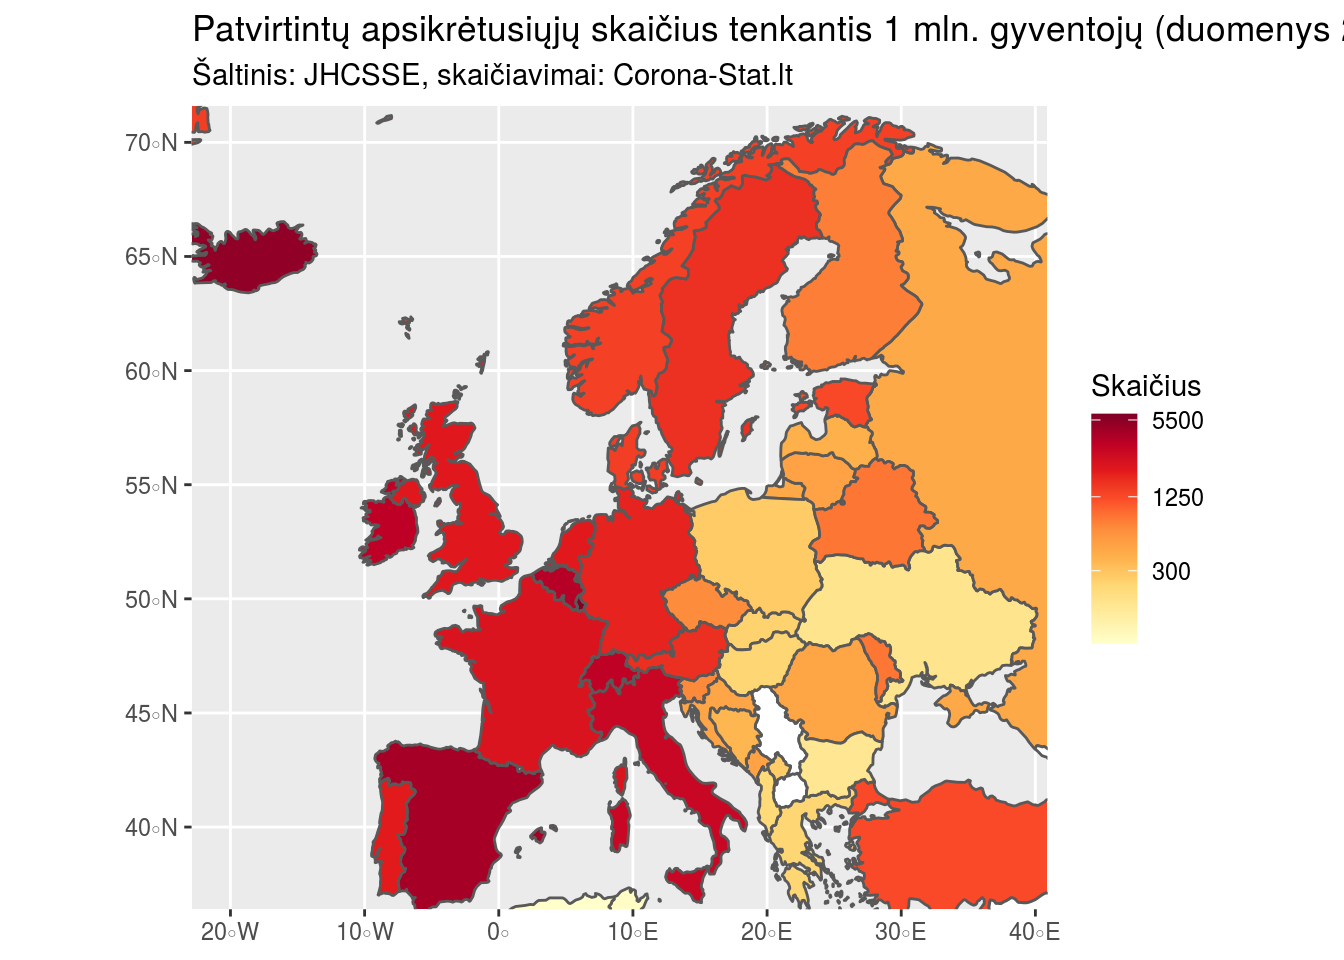
\includegraphics[scale=0.575]{eu_map.png}
\end{frame}


\begin{frame}{Covid situacija - Lietuva}
2020-04-23 LT: 7401 testas, 12 teigiamų

\centering
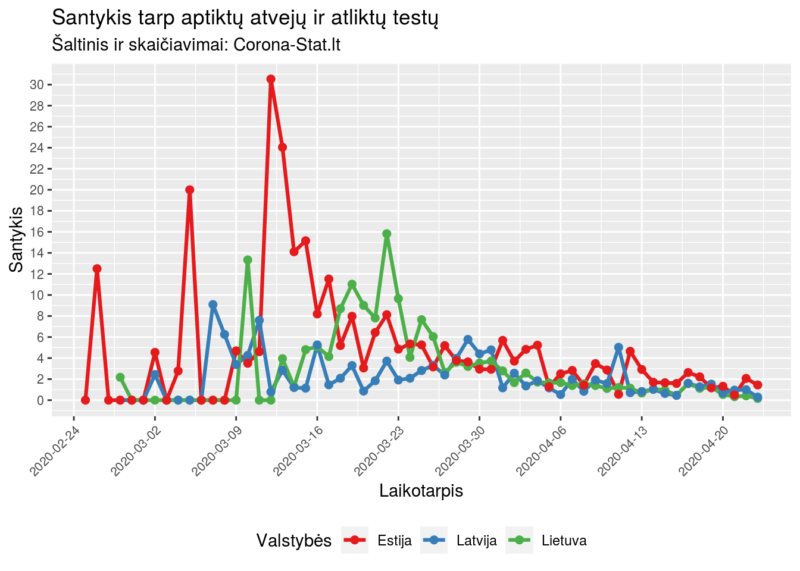
\includegraphics[scale=0.375]{balt.png}
\end{frame}

\begin{frame}{Apple maps užklausos}
\centering
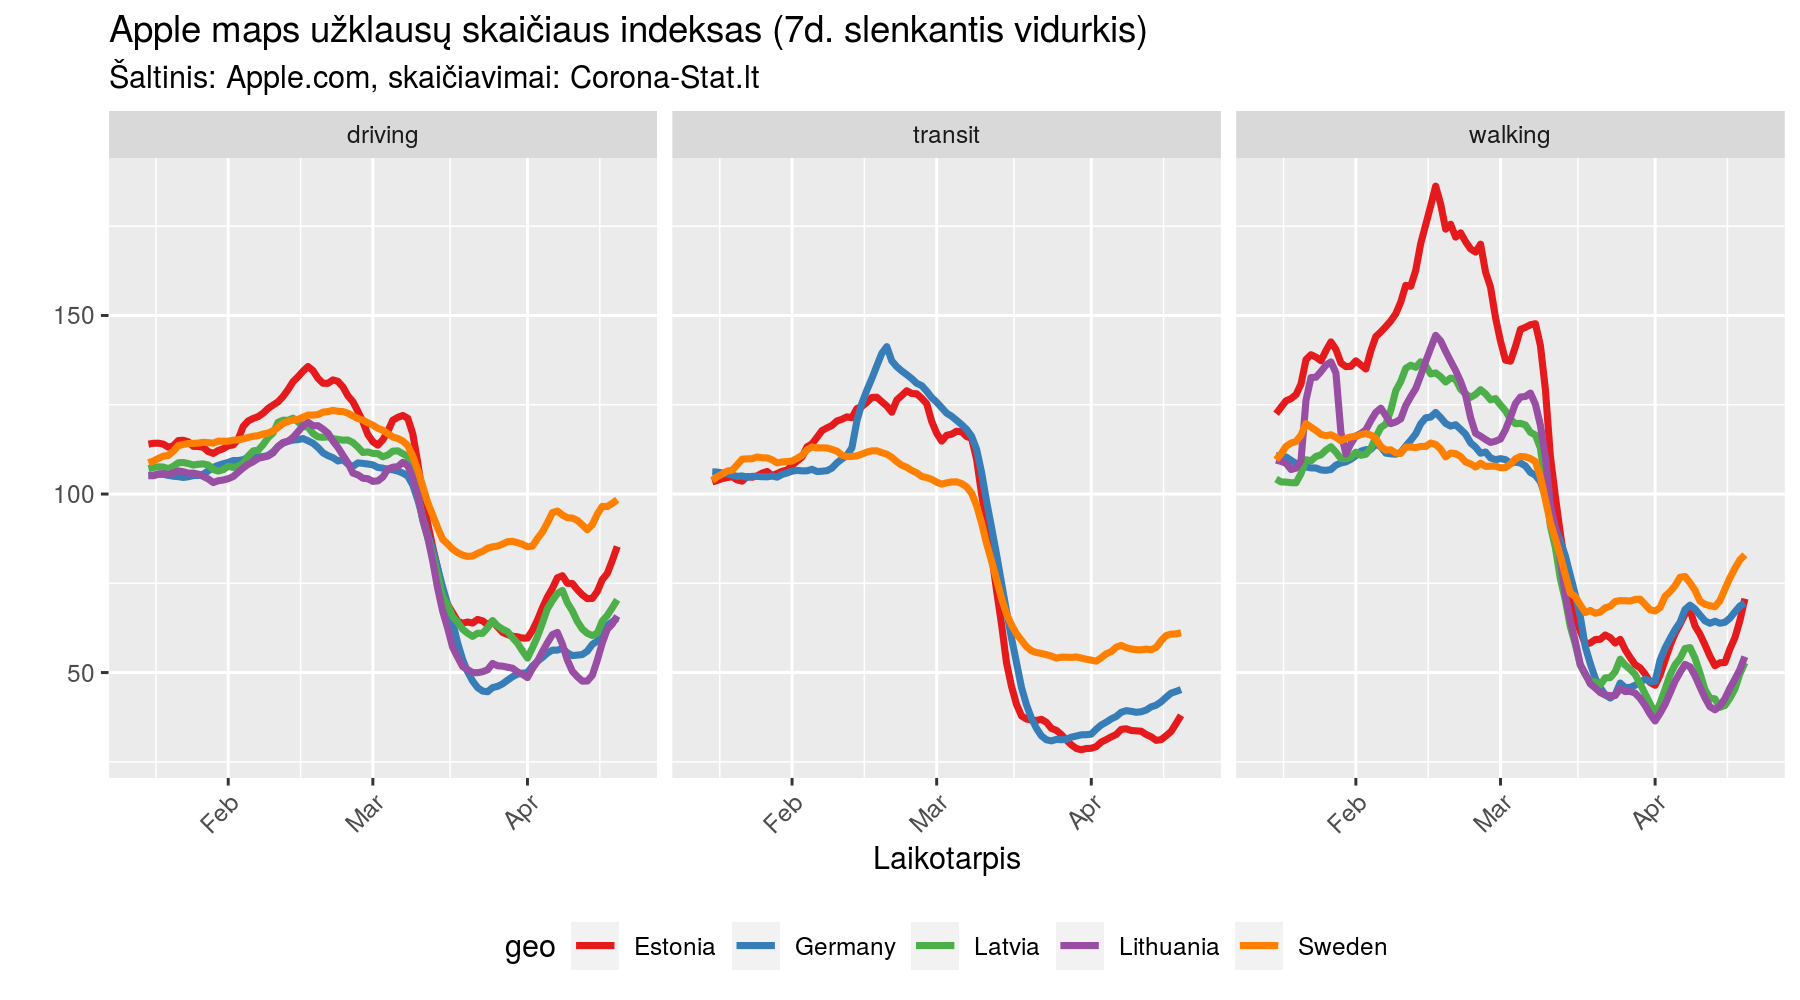
\includegraphics[scale=0.575]{apple_judejimas.png}
\end{frame}

\begin{frame}{Apple maps užklausos}
\centering
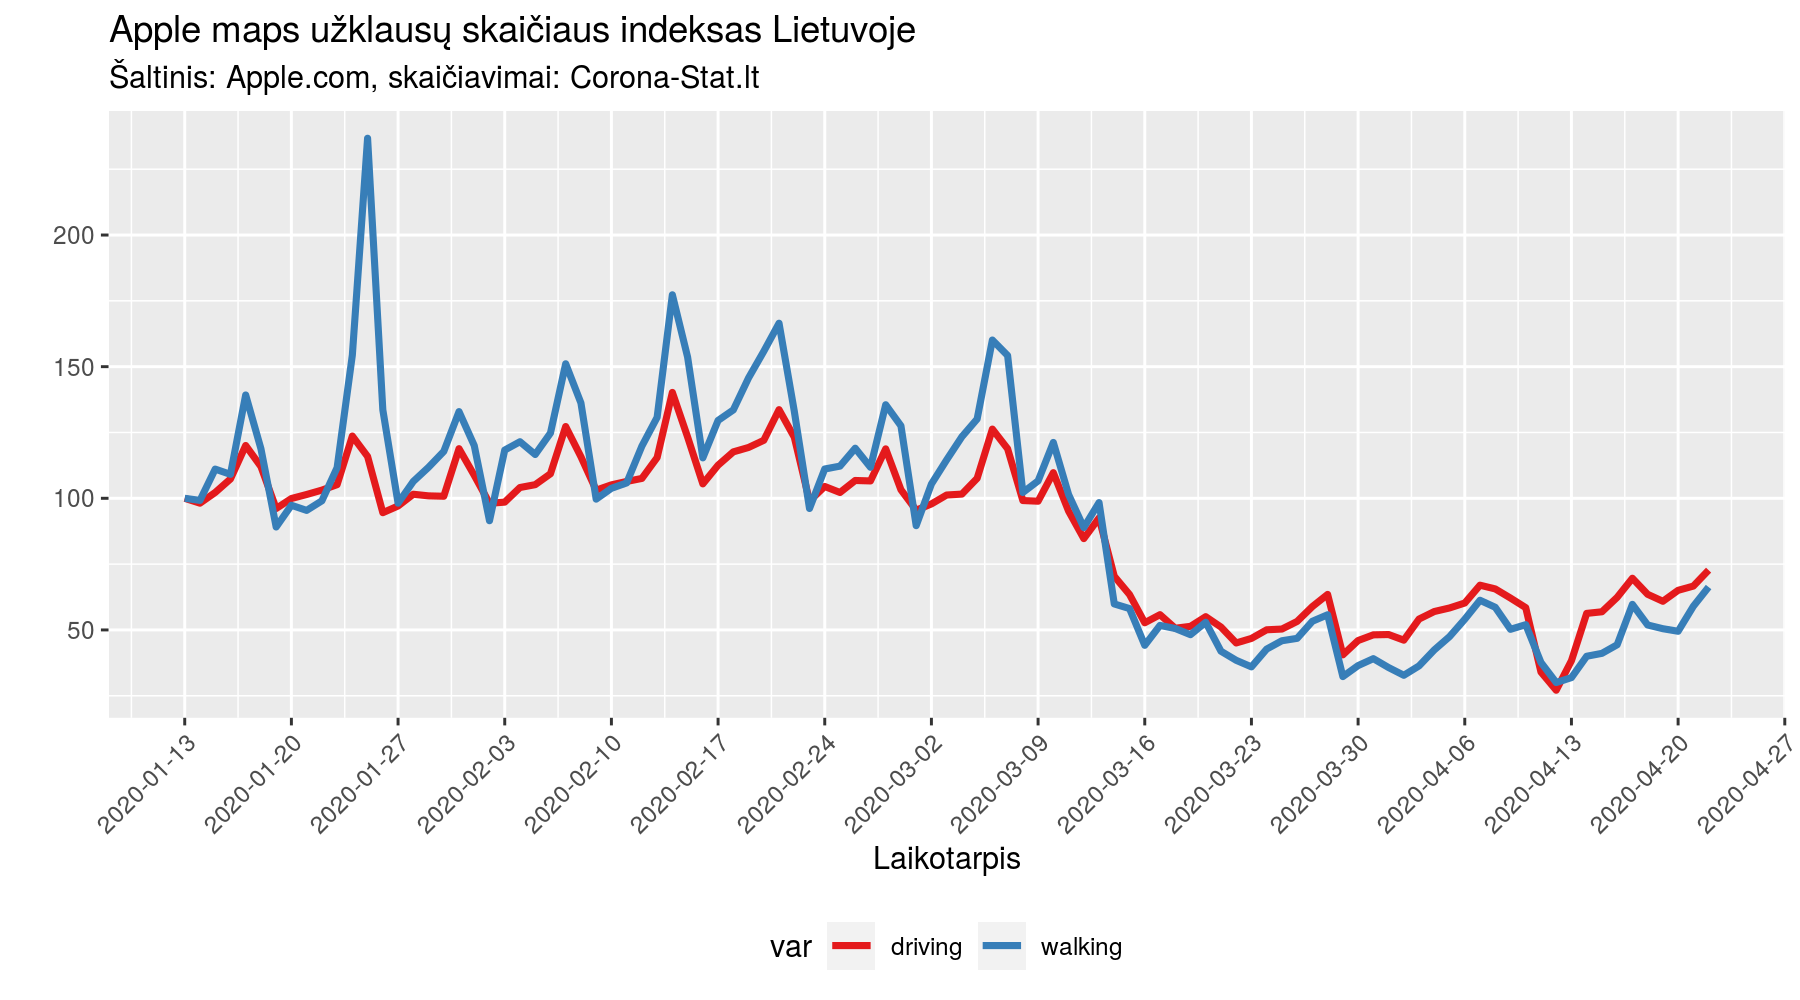
\includegraphics[scale=0.575]{apple_judejimas_lt.png}
\end{frame}

\section{Covid pasekmės}
\subsection{Darbo rinka}

\begin{frame}
\begin{LARGE}
Darbo rinka
\end{LARGE}
\end{frame}

\begin{frame}{Grupės darbuotojų atleidimai}
\centering
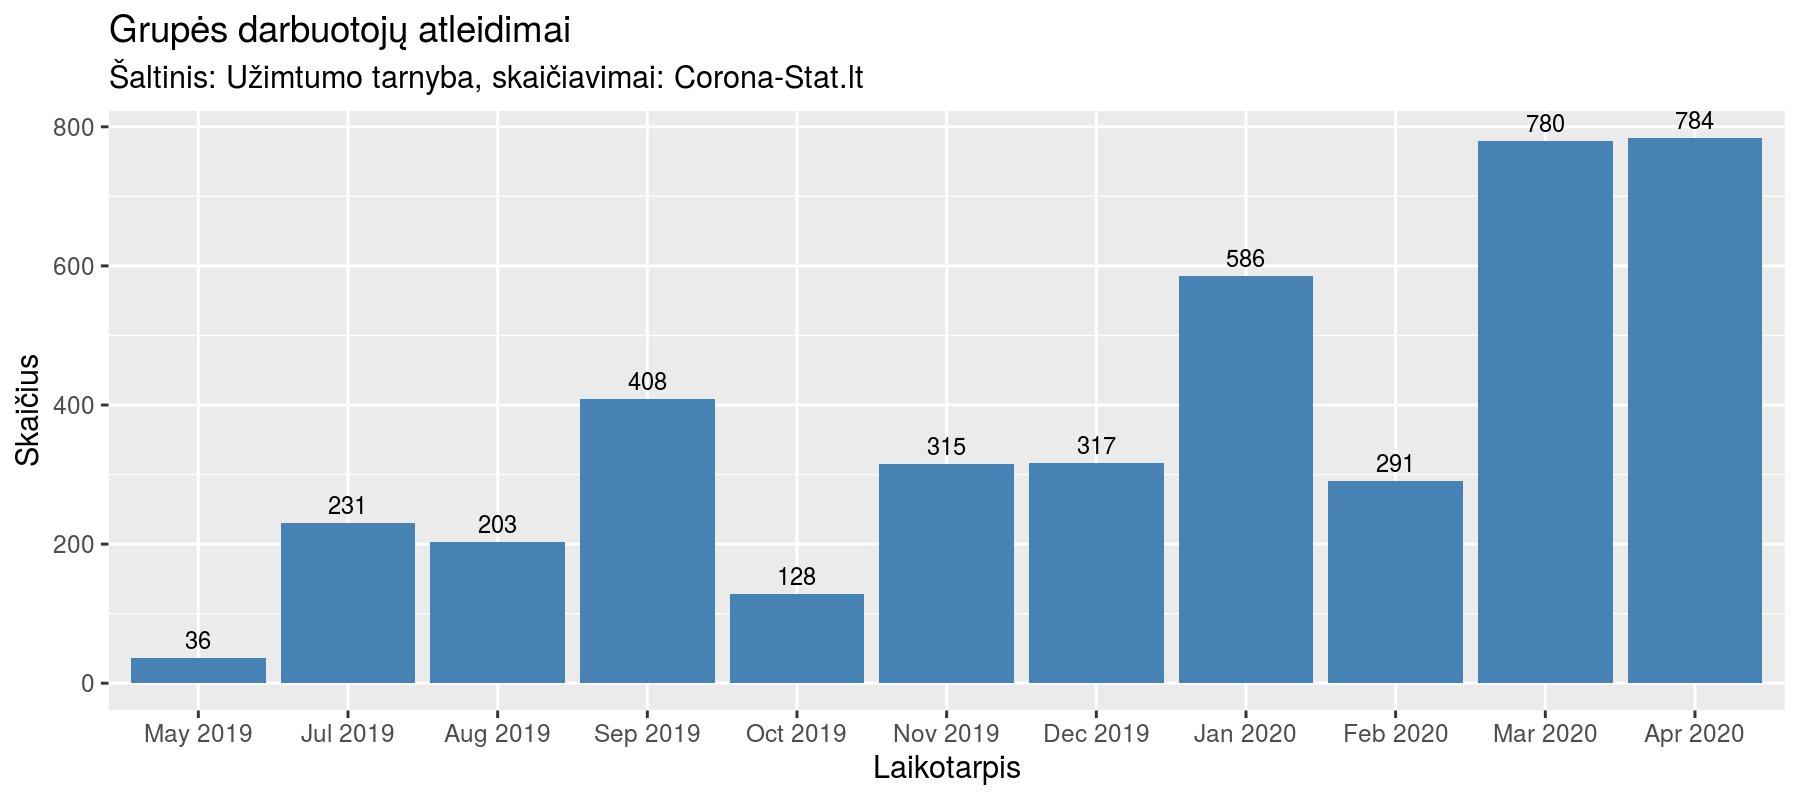
\includegraphics[scale=0.5]{grupes_darbuotoju_atleidimai_men_sum.png}
\begin{footnotesize}
\begin{itemize}
\item Keleivinis oro transportas	420
\item Drabužiai + avalynė 239 (“UTENOS TRIKOTAŽAS” - 84)
\item Baldų gamyba	87
\item Konsultacinė verslo veikla	83
\end{itemize}
\end{footnotesize}
\end{frame}


%\begin{frame}{Grupės darbuotojų atleidimai}
%Grupės darbuotojų atleidimai nuo 2020 vasario mėn.
%\input{grupiniai_atleidimai.txt}
%\end{frame}

\begin{frame}{Bedarbių skaičius}
\centering
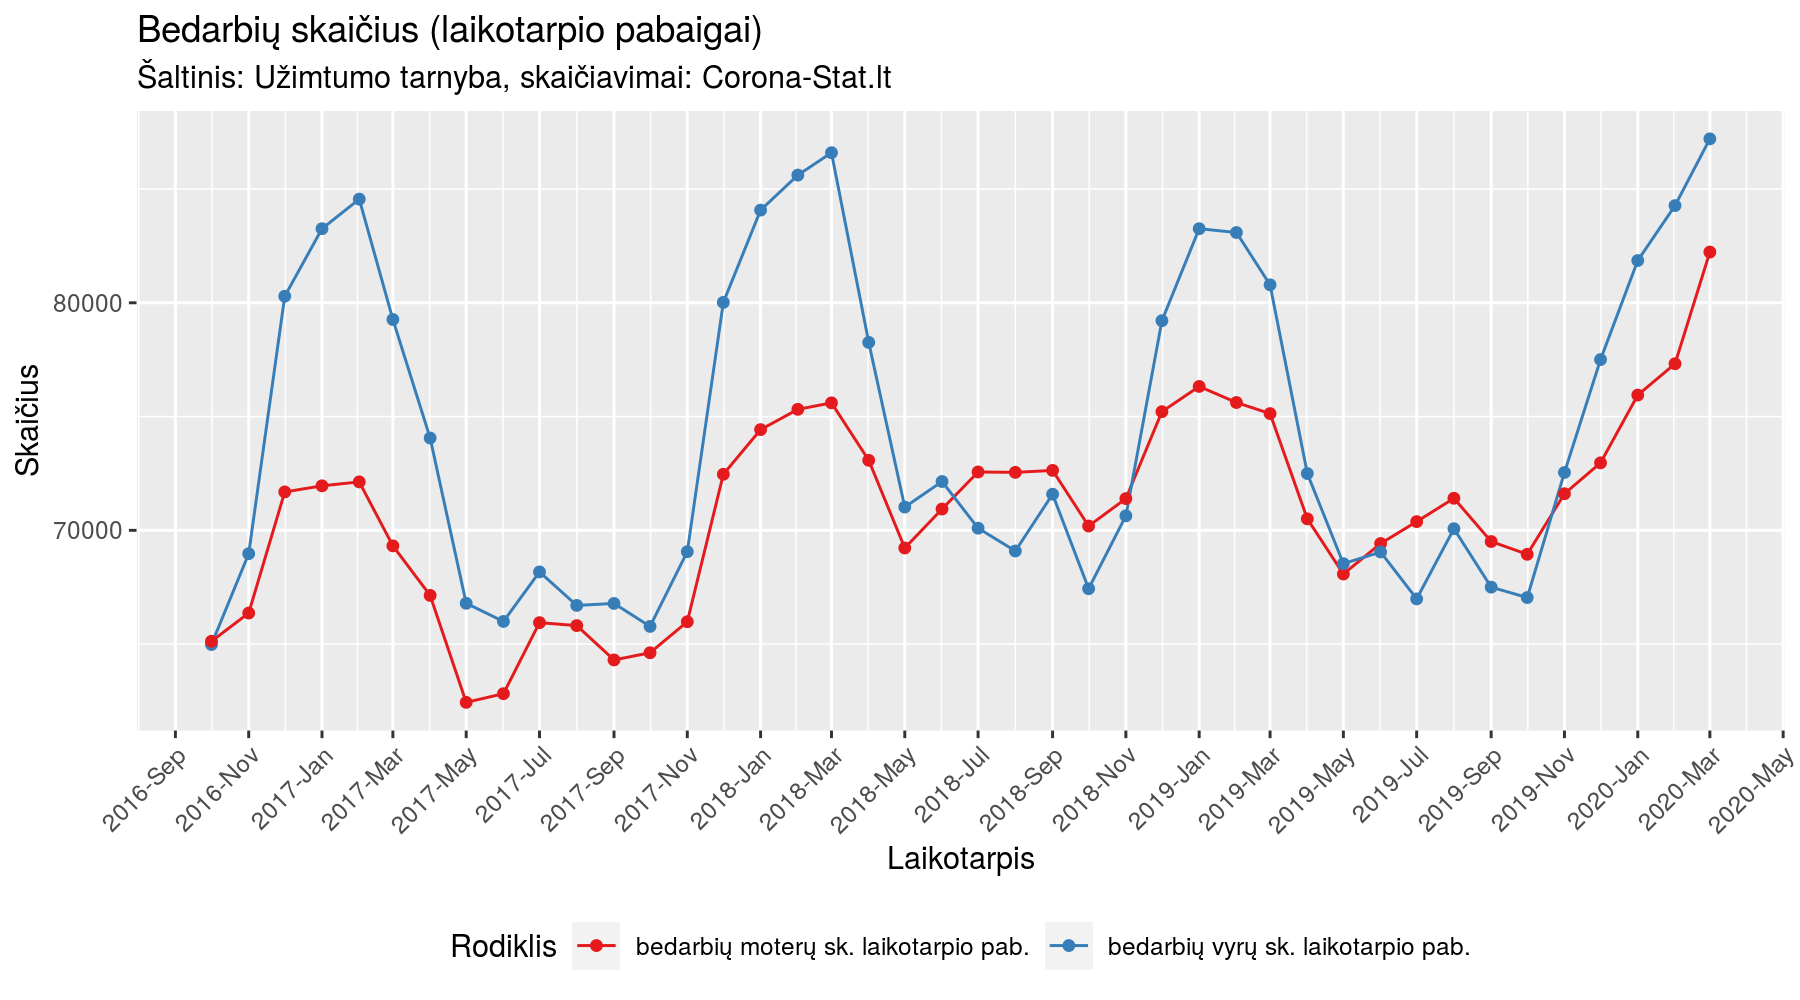
\includegraphics[scale=0.575]{bedarbiu_sk.png}
\end{frame}

%\begin{frame}{Bedarbių proc. nuo DAG}
%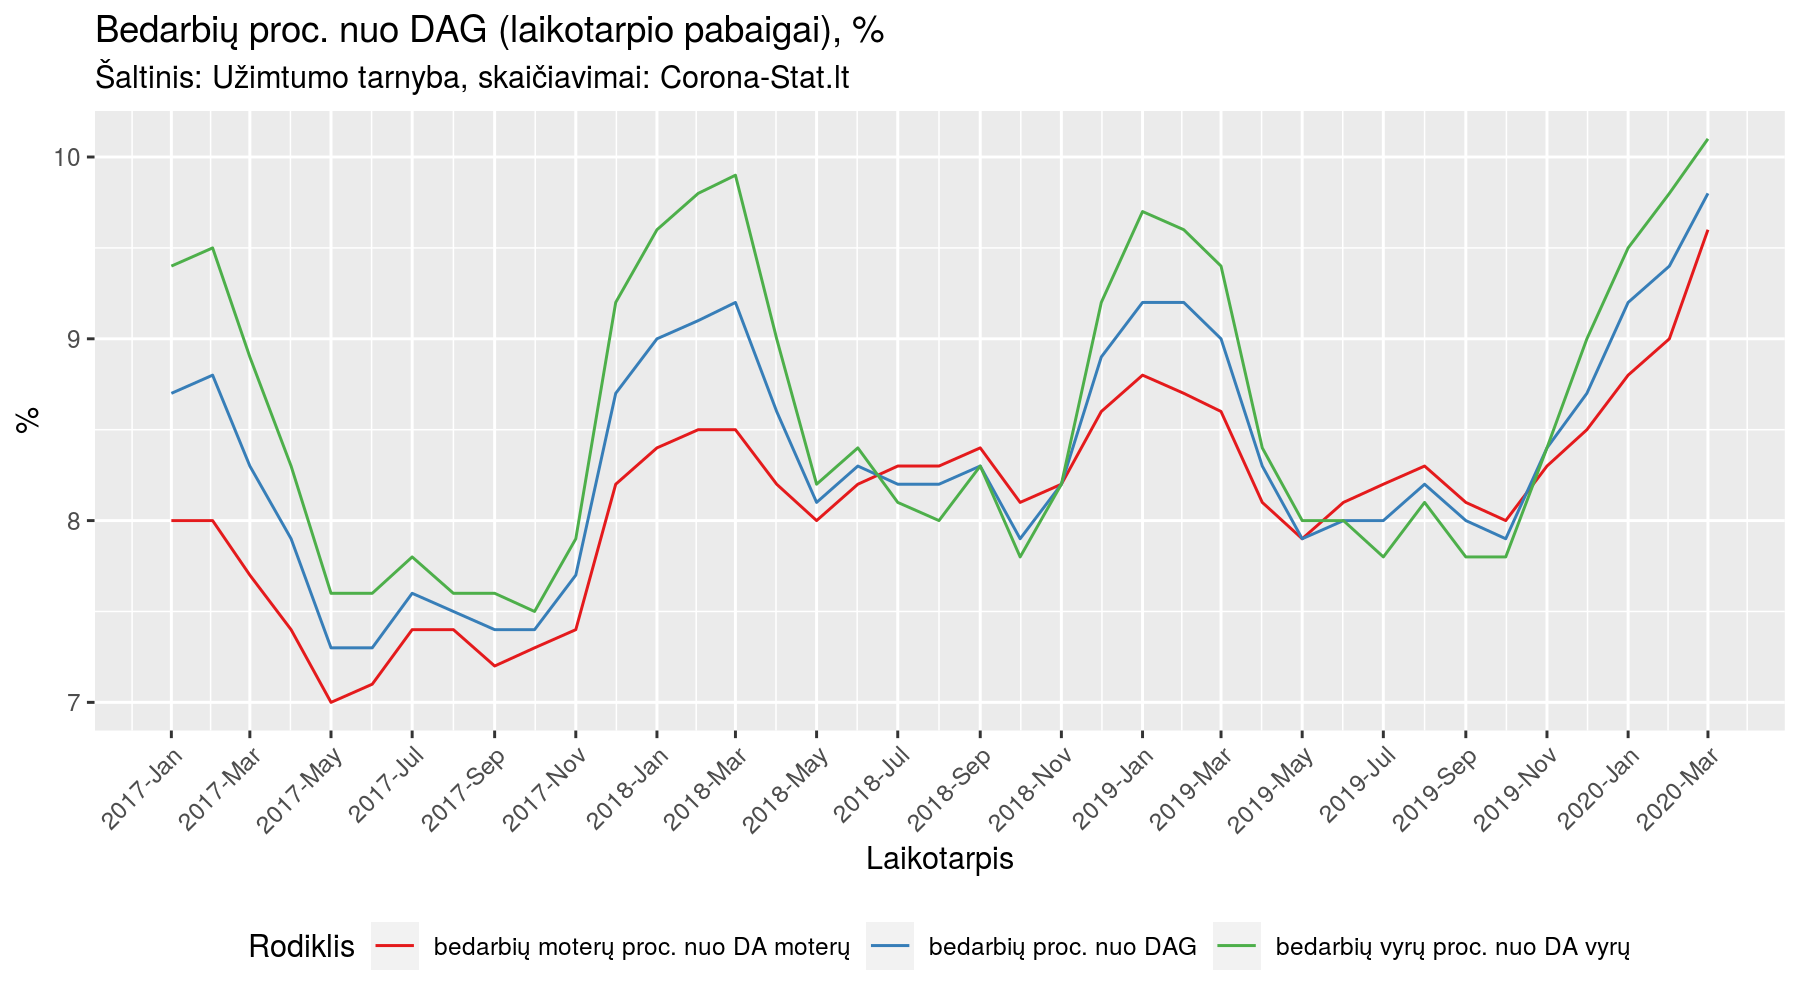
\includegraphics[scale=0.5]{bedarbiu_proc.png}
%\end{frame}

\subsection{Kainos, poveikis vartotojams}

\begin{frame}
\begin{LARGE}
Kainos, poveikis vartotojams
\end{LARGE}
\end{frame}

\begin{frame}{Eurozonos metinė infliacija}
\centering
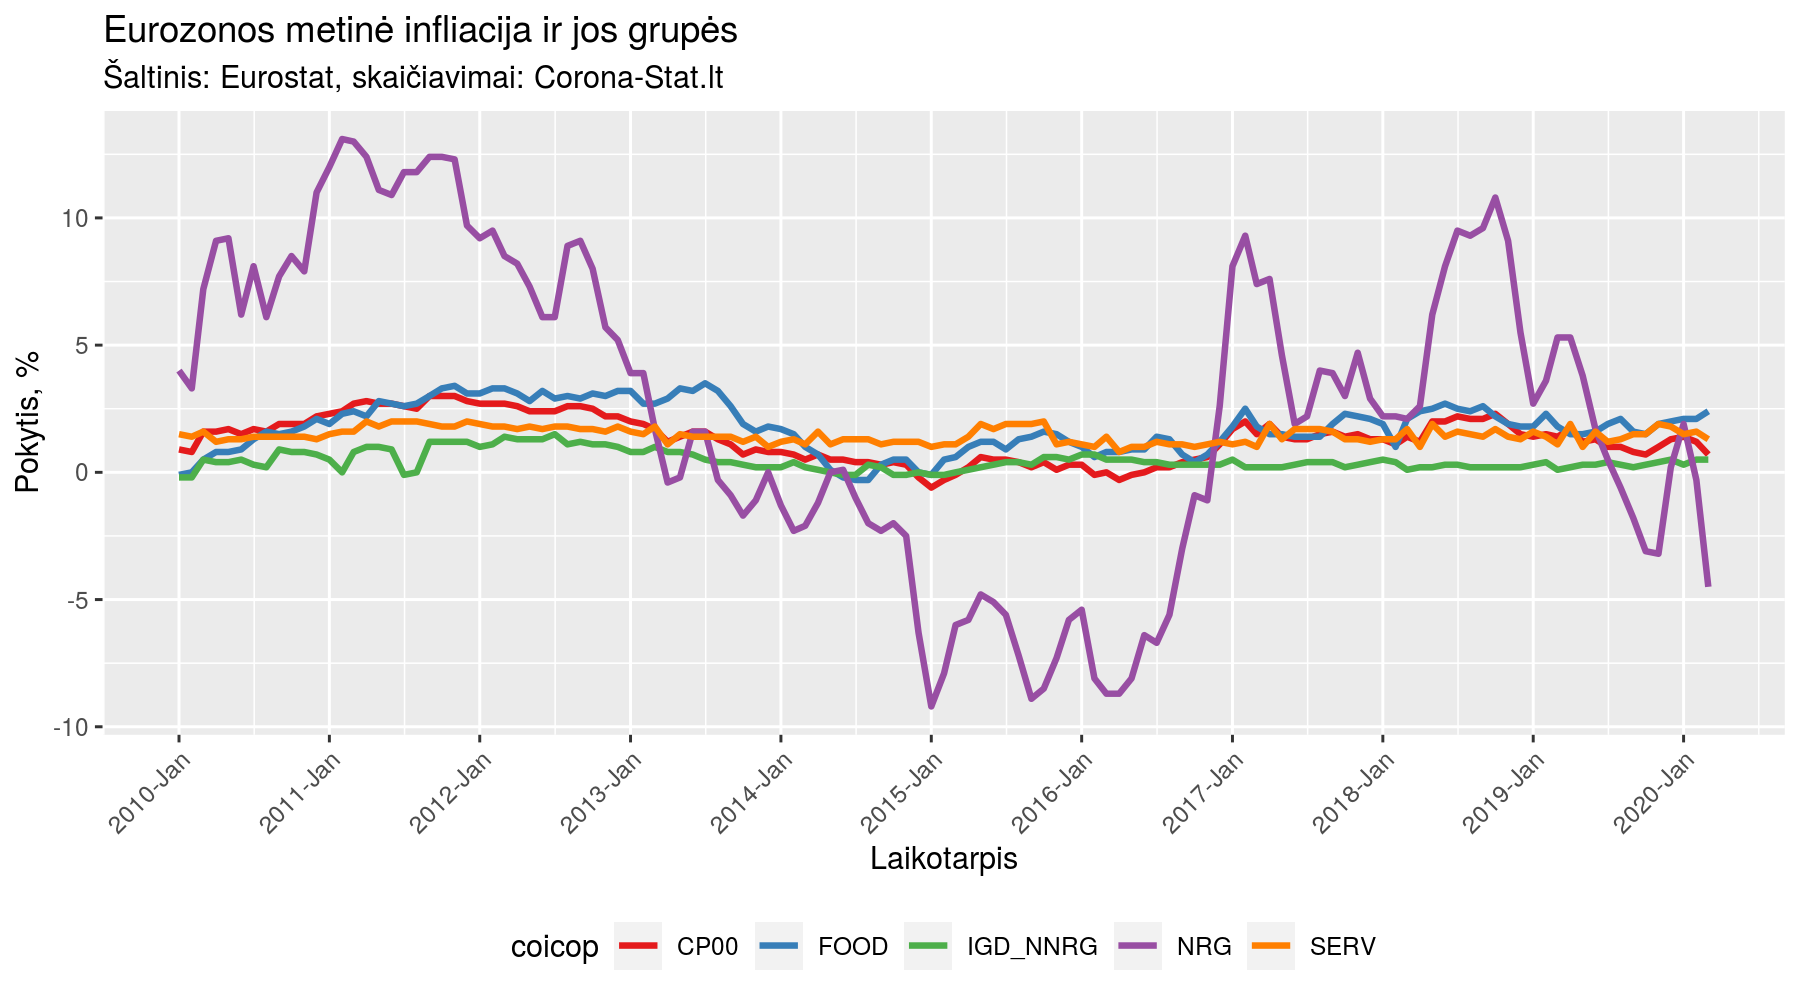
\includegraphics[scale=0.575]{infliacija_ez.png}
\end{frame}

\begin{frame}{Eurozonos metinė infliacija}
\centering
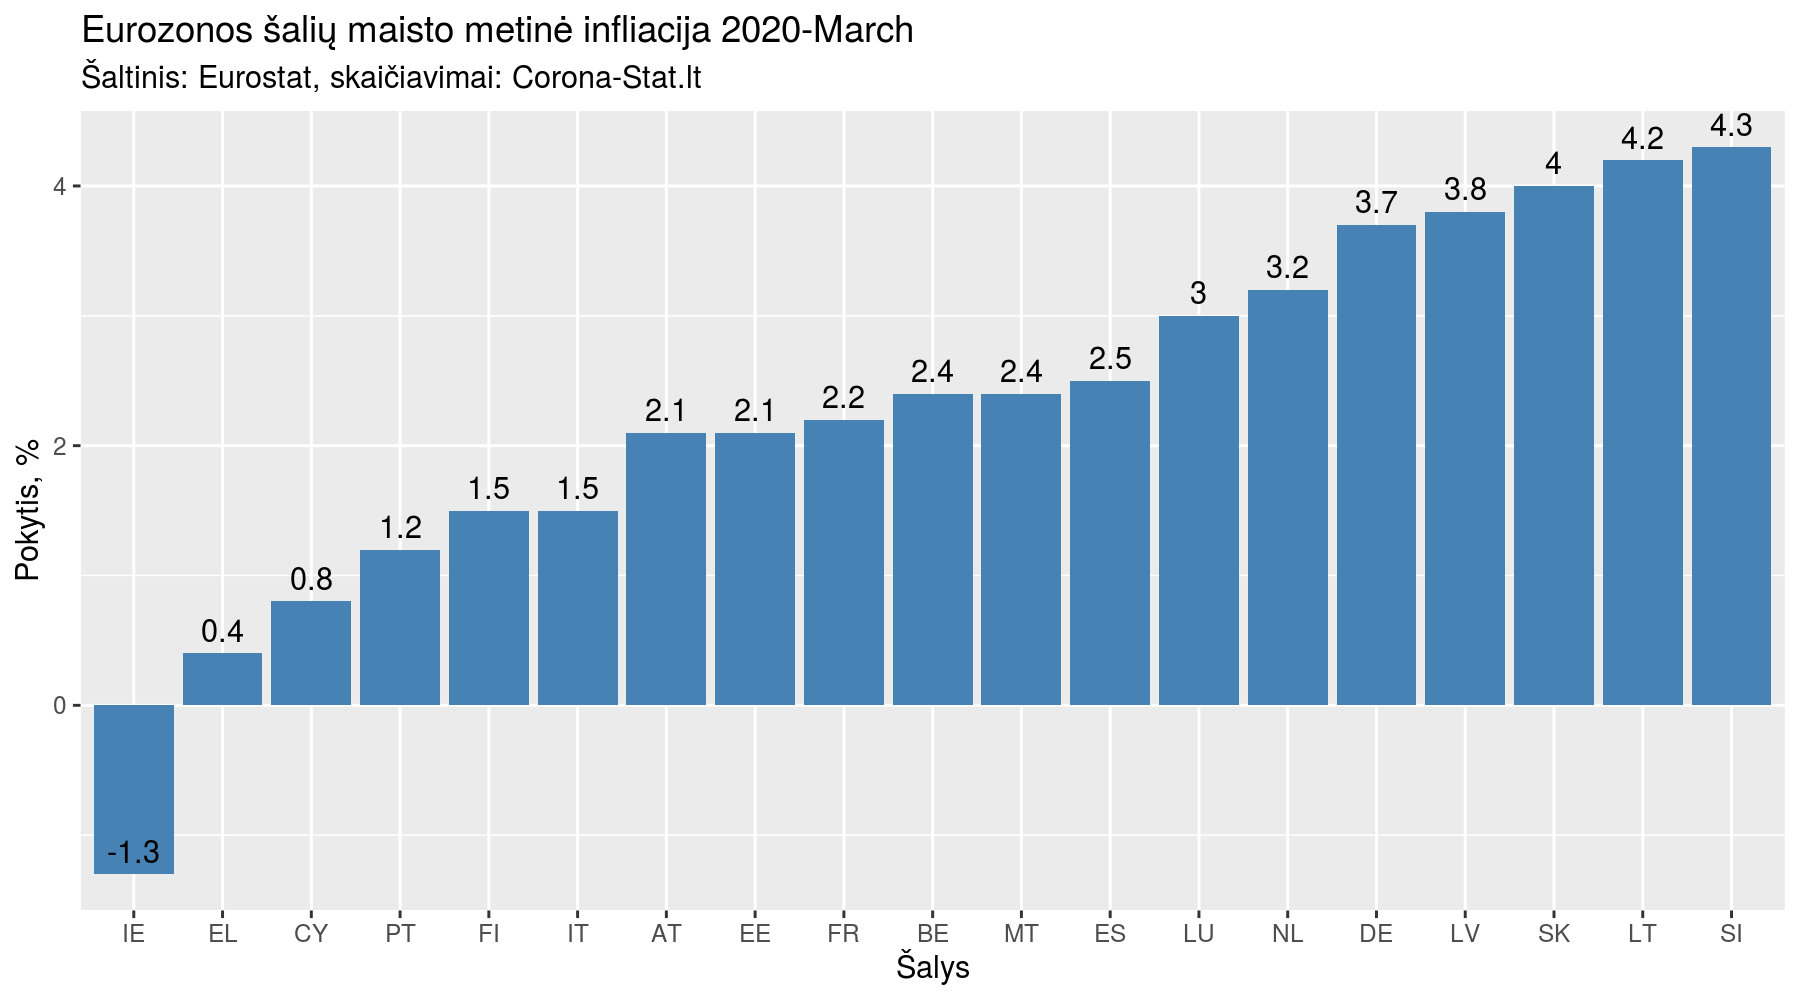
\includegraphics[scale=0.575]{infliacija_maistas.png}
\end{frame}

%\begin{frame}{Eurozonos metinė infliacija}
%\centering
%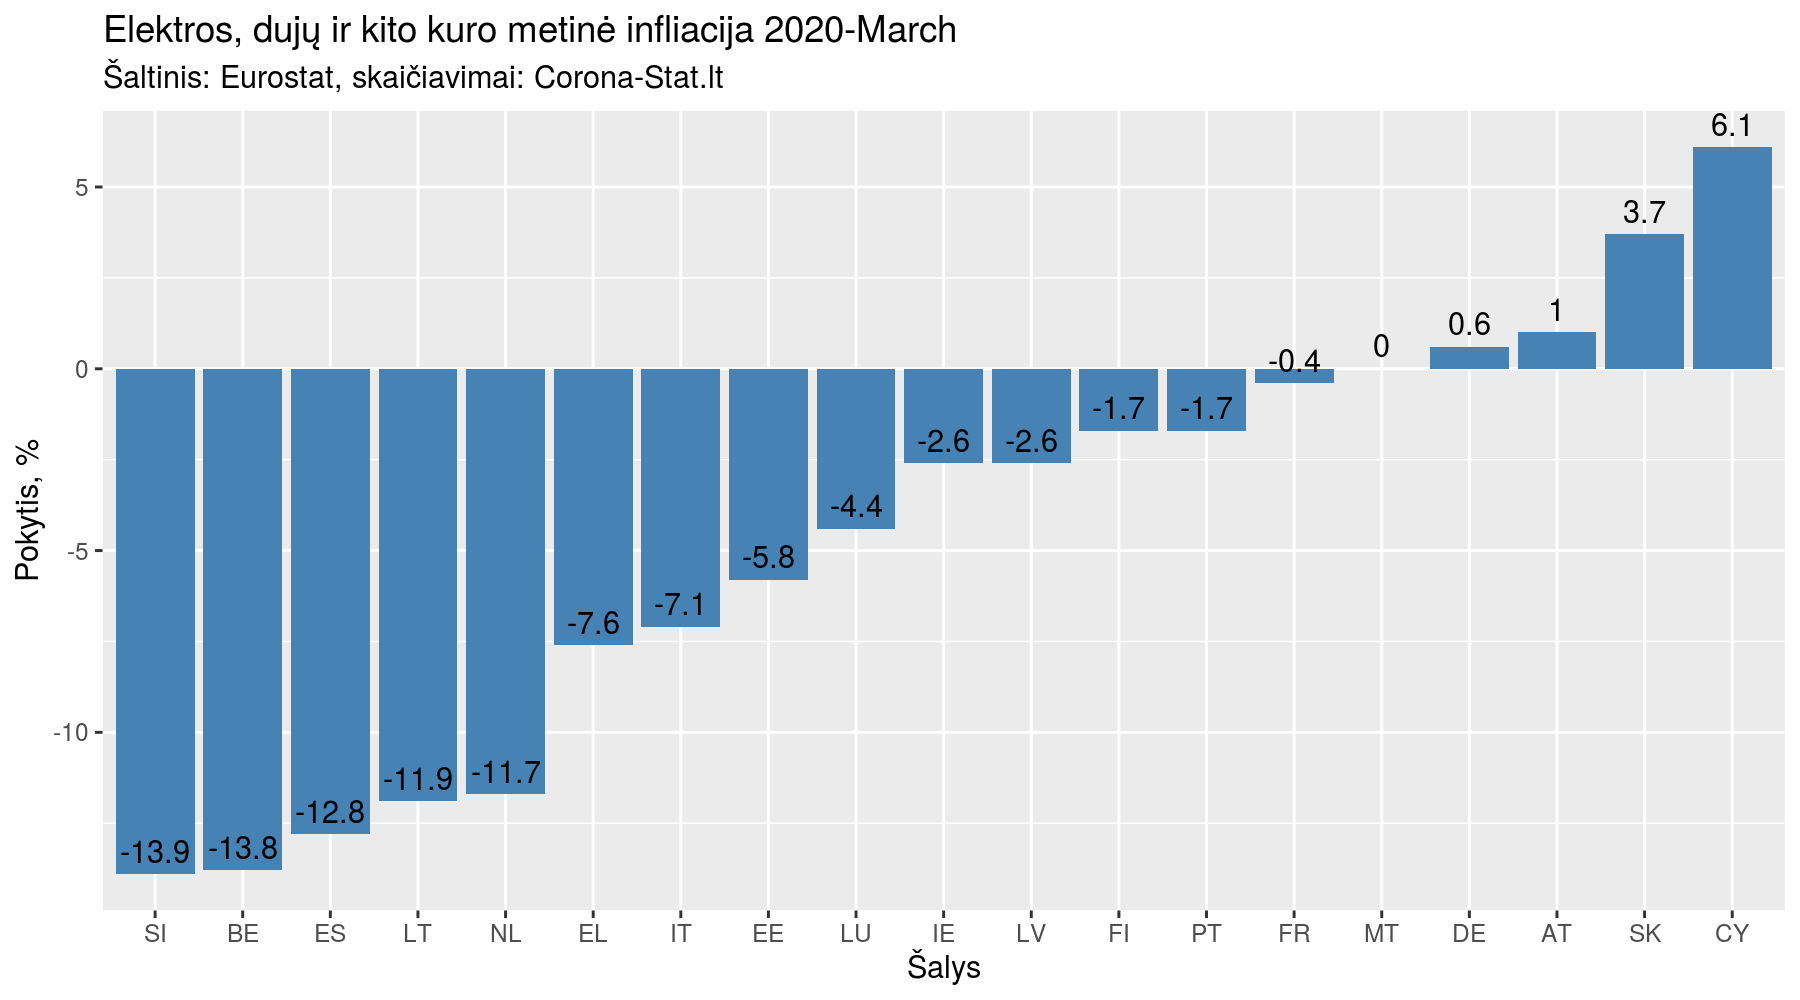
\includegraphics[scale=0.575]{infliacija_elektra_dujos.png}
%\end{frame}


\begin{frame}{Eurozonos metinė infliacija}
\centering
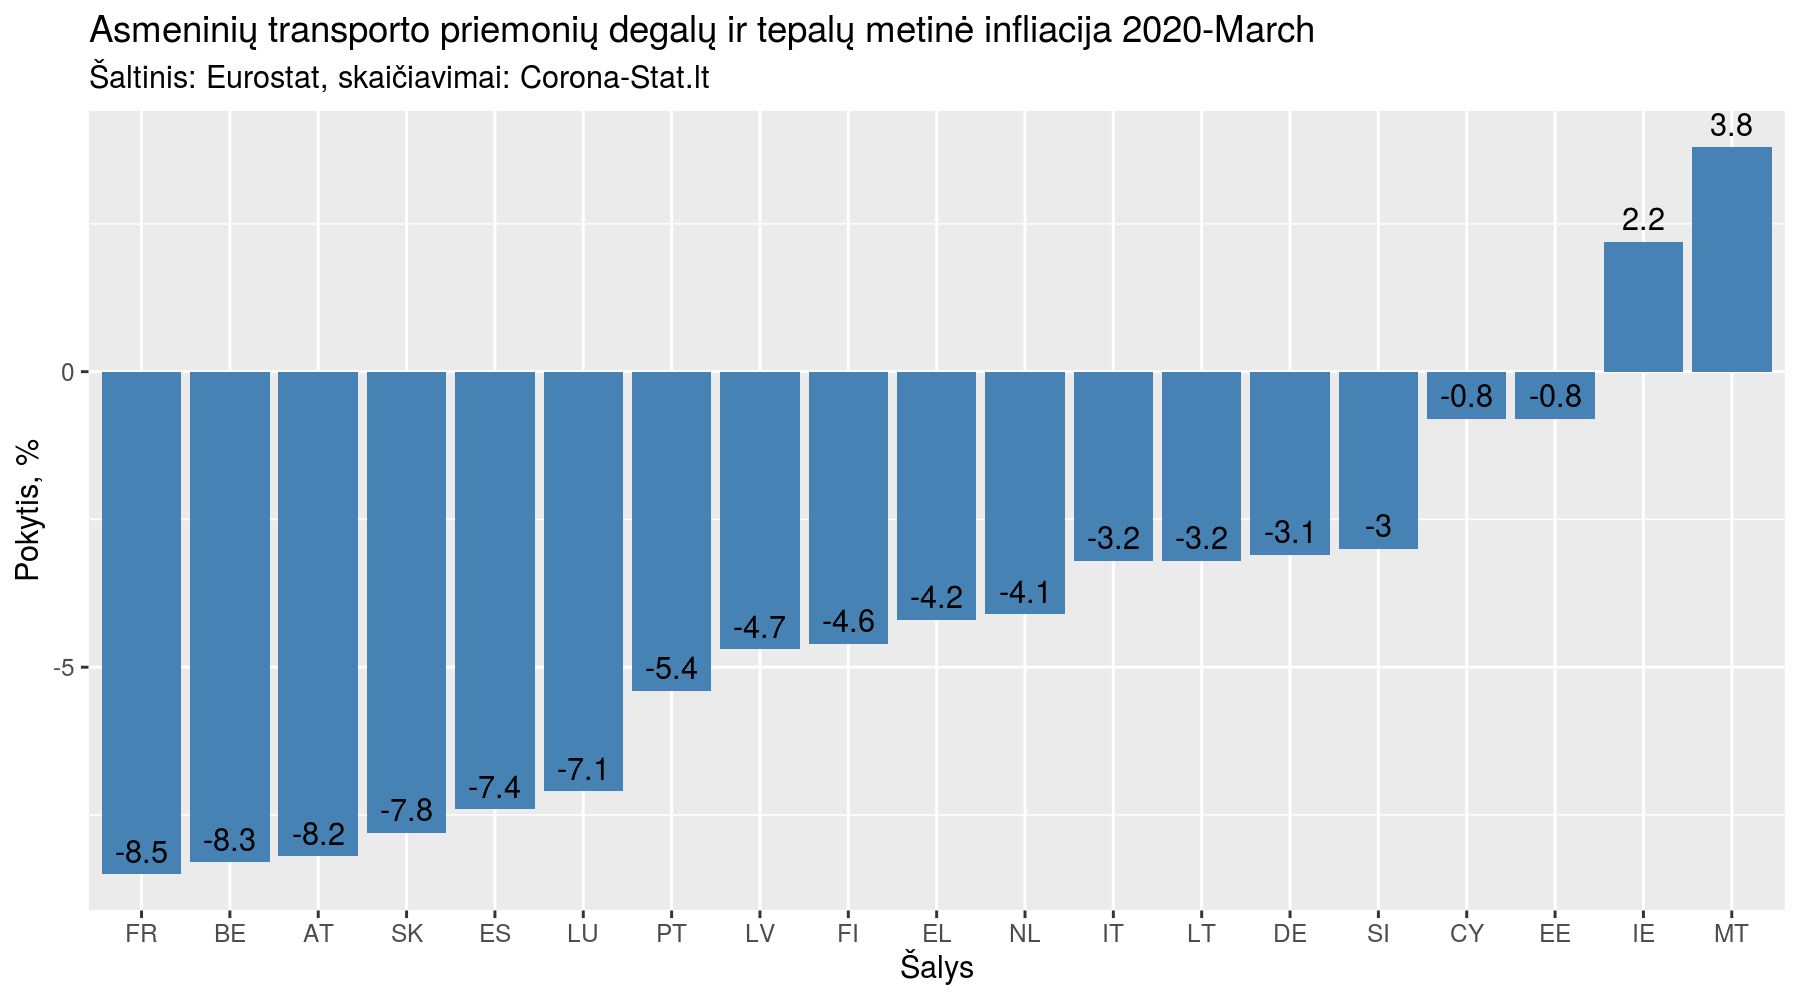
\includegraphics[scale=0.575]{infliacija_degalai.png}
\end{frame}

\subsection{Pramonė, lūkesčiai ir eksporto rinkos}

\begin{frame}
\begin{LARGE}
Pramonė, lūkesčiai ir eksporto rinkos
\end{LARGE}
\end{frame}

\begin{frame}{Lietuva maža ir atvira ekonomika}
\centering
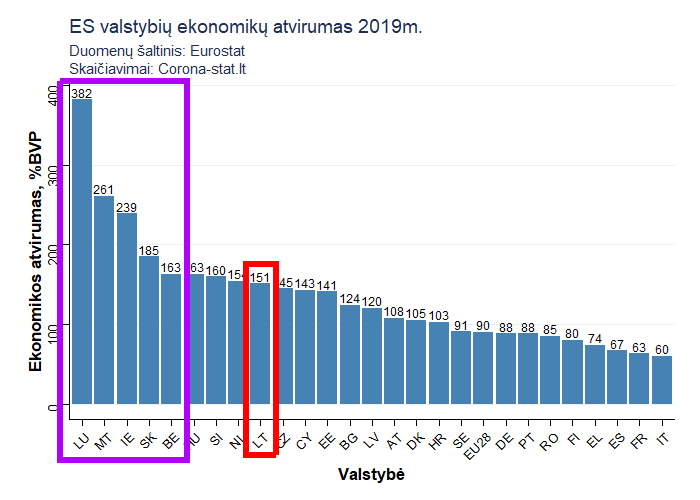
\includegraphics[scale=0.45]{atvirumas.png}
\end{frame}



\begin{frame}{Verlso lūkesčiai kaip vedantieji (lead) inkdikatoriai}
\begin{scriptsize}
\end{scriptsize}
\centering
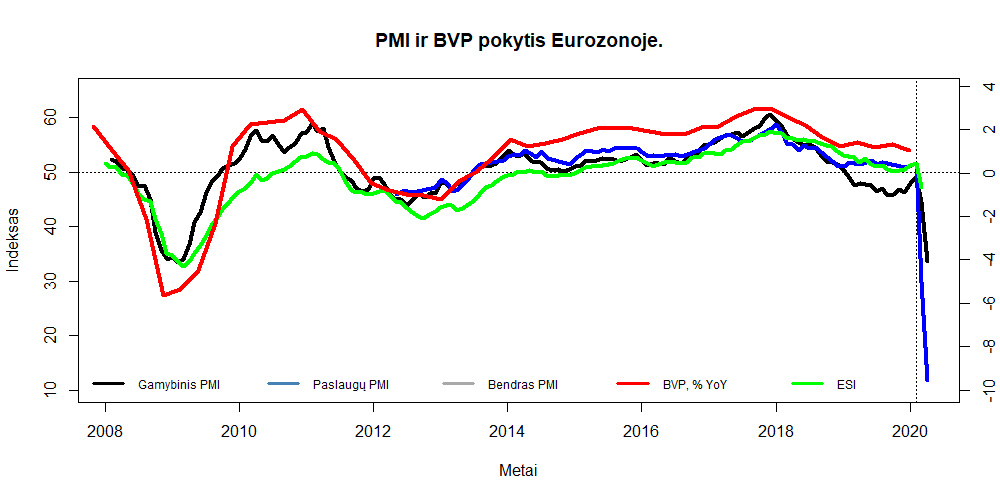
\includegraphics[scale=0.575]{Rplot07.png}
\end{frame}

\begin{frame}{Nepaisant milžiniškų skatinimo paketų...}
\centering
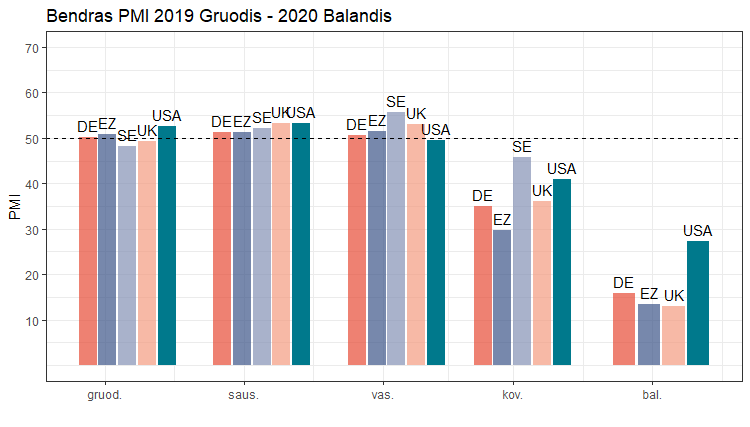
\includegraphics[scale=0.65]{Rplot06.png}
\end{frame}

\begin{frame}{Situacija Lietuvoje}
\begin{itemize}
\item LPK duomenimis:
\begin{itemize}
\item 40\% LPK narių sustabdė veiklą
\item 100 tūkst. darbuotojų prastovose
\item Lėtas pagalbos suteikimas: patenkinta 2.200 iš 30.000 prašymų
\end{itemize}
\item Invegos pagalba: panaudoti 2 \% numatytų 1.3 mlrd. lėšų
\item Prievolė išlaikyti darbo vietas (gaunant prastovos subsidiją) gąsdina smulkiuosius
\item FinMin prognozuoja 2020m.:
\begin{itemize}
\item LT BVP -2.8\% (EZ -2.5\%)  arba 7.3\% (EZ -5 \%)
\item LT eksportas: -6.6 \% arba -15 \%
\end{itemize}
\item TVF: EZ 2020m. -7.5\%
\end{itemize}
\end{frame}



\subsection{Naftos rinka ir geopolitika}

\begin{frame}
\begin{LARGE}
Naftos rinka ir geopolitika
\end{LARGE}
\end{frame}


\begin{frame}{Naftos paklausa ir karas dėl Kinijos}
Naftos rinka – dviguboje krizėje:
\begin{itemize}
\item Dėl stojančios ekonomikos mažėja pasaulinė naftos paklausa
\begin{itemize}
\item Naftos paklausa ir pasiūla - neelastinga kainos atžvilgiu
\end{itemize}
\item Tarp naftos gavybos šalių vyksta karas dėl ateities rinkų
\begin{itemize}
\item D.Trump bandymas inicijuoti gavybos mažinimą - bandymas išgelbėti savo rinkimus
\item Saudo Arabijos ir Rusijos kainų karas
\item Didžiausias laimėtojas - Kinija
\item Balandžio 12d. OPEC+ susitarė dėl 9.7 mln barelių (~10 proc. visos gavybos)
\end{itemize}
\end{itemize}
\end{frame}


\begin{frame}{Naftos ir dujų kainų raida}
\centering
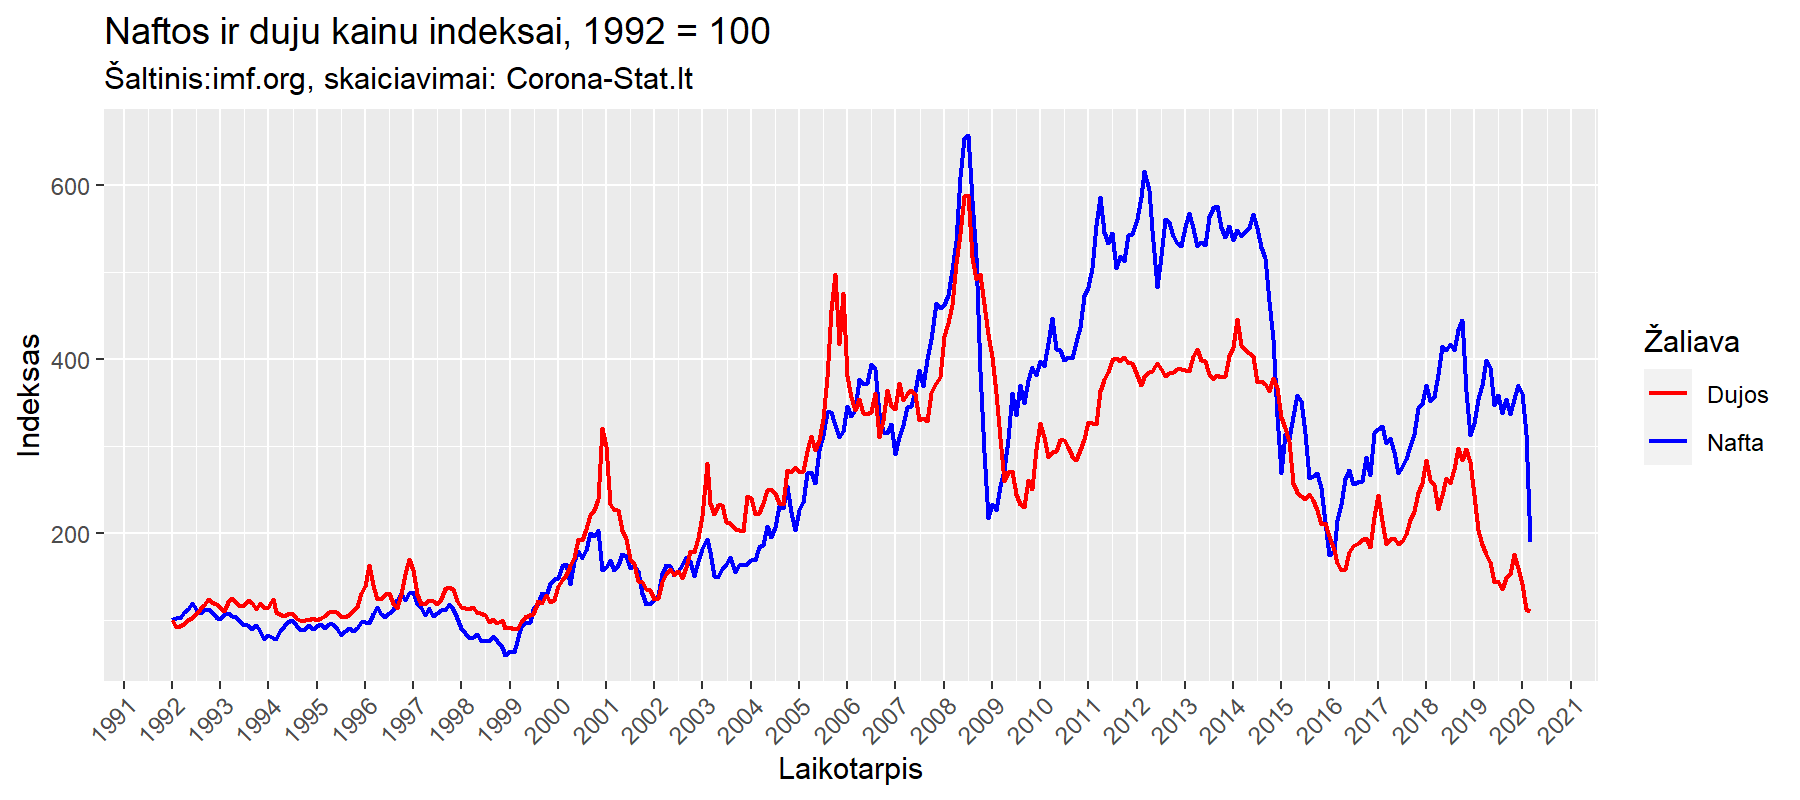
\includegraphics[scale=0.65]{naftos_kainos_monthly.png}
\end{frame}

\begin{frame}{WTI spekuliacijos burbulo sprogimas}
\centering
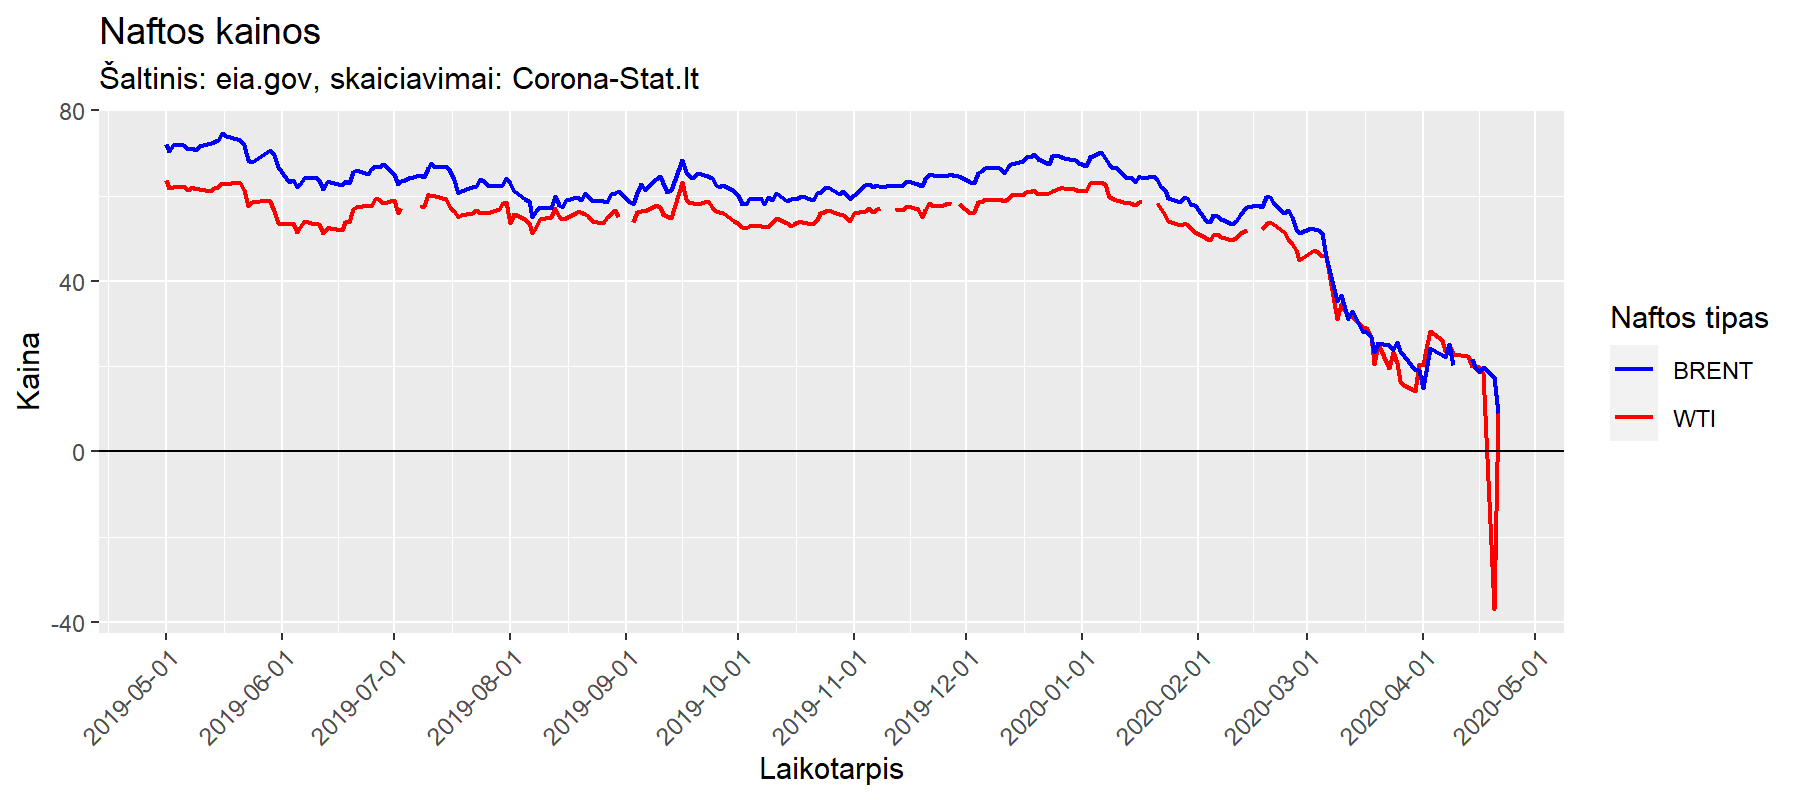
\includegraphics[scale=0.65]{naftos_kainos_daily.png}
\end{frame}

\begin{frame}{Naftos kainų poveikis}
Lietuvoje:
\begin{itemize}
\item Elektra atpigs 22 \%
\item Dujos namų ūkiams - 15-22 \%
\item Bendras kainų mažėjimas (pvz., maisto produktų)
\item Sąlyginė pagalba Achemai - didžiausiai pramoninei dujų vartotojai Lietuvoje
\end{itemize}
Globaliai:
\begin{itemize}
\item mažesnės investicijos į atsinaujinančią energetiką
\item galimos didesnės geopolitinės įtampos (pvz., Rusija)
\item dar mažiau JAV dėmesio Artimiesiems rytams ir daugiau dėmesio Pietryčių Azijai
\item galimai keisis ES biudžeto prioritetai (mažiau Green Deal)
\end{itemize}
\end{frame}


\begin{frame}{Coronabonds vs ESM}
\centering
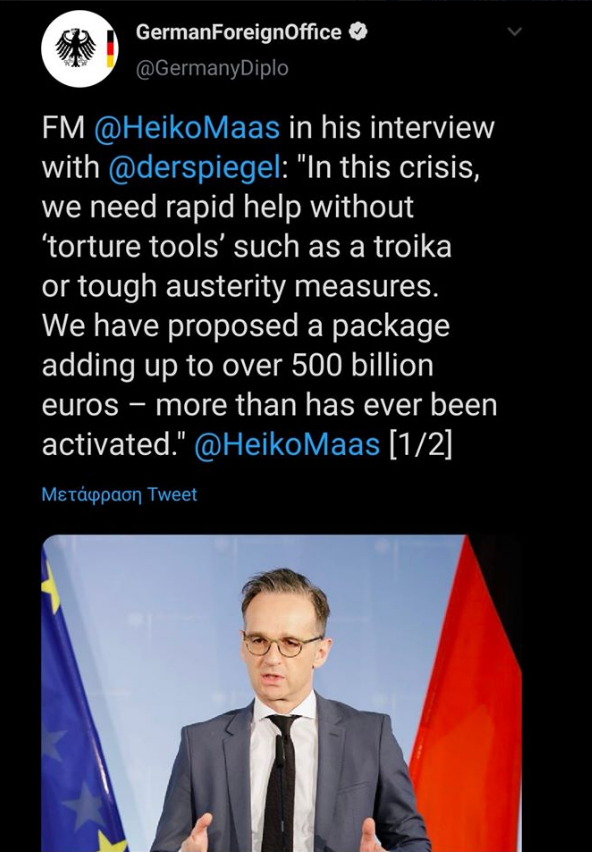
\includegraphics[scale=.25]{maas.png}

\end{frame}

\begin{frame}
\begin{LARGE}
Klausimai - atsakymai
\end{LARGE}
\end{frame}


\end{document}